\documentclass[9pt,aspectratio=169]{beamer}


\usepackage{tabu, booktabs, multirow}
\usepackage{tabularx}
\usepackage{multicol}
\usepackage{setspace}
\usepackage[official]{eurosym}
\usepackage{graphicx}

\usepackage{hyperref}
\hypersetup{
    colorlinks=true,
    linkcolor=blue,
    filecolor=magenta,      
    urlcolor=cyan,
    pdftitle={EC3318/MN3101 Lecture 3},
    pdfpagemode=FullScreen,
    }

\urlstyle{same}

\graphicspath{ {./pix_l3/} }



\newcolumntype{Y}{>{\centering\arraybackslash}X}  % Centered version of X

\newcommand{\placeholderbox}[1]{%
  \begin{center}
    \fbox{\parbox[c][0.5\textheight][c]{0.9\linewidth}{\centering \textit{#1}}}
  \end{center}
}
% St Andrews Color Palette

% Blues
\definecolor{StAndrewsLightBlue}{RGB}{0,174,239}
\definecolor{StAndrewsMidBlue}{RGB}{0,125,197}
\definecolor{StAndrewsBlue}{RGB}{0,83,155}  % Previously defined

% Reds
\definecolor{StAndrewsBurgundy}{RGB}{198,12,70}
\definecolor{StAndrewsRed}{RGB}{238,49,42}  % Previously defined

% Purple
\definecolor{StAndrewsPurple}{RGB}{123,67,154}

% Orange
\definecolor{StAndrewsOrange}{RGB}{245,132,43}

% Greens
\definecolor{StAndrewsGreen}{RGB}{84,185,72}
\definecolor{StAndrewsMidGreen}{RGB}{0,133,63}
\definecolor{StAndrewsDarkGreen}{RGB}{0,89,83}

% Yellow
\definecolor{StAndrewsYellow}{RGB}{255,223,0}

% Black
\definecolor{StAndrewsBlack}{RGB}{35,31,32}

\setbeamercolor*{structure}{fg=StAndrewsBlack}
\setbeamercolor{title}{fg=StAndrewsBlack}
\setbeamercolor{title separator}{fg=StAndrewsBlue}
\setbeamercolor{frametitle}{bg=StAndrewsBlue, fg=white}

\usetheme{metropolis}
\usepackage{tikz}
\usetikzlibrary{calc}
\usetikzlibrary{arrows.meta, positioning, shapes.geometric, shadows}
\usepackage[export]{adjustbox}
\usepackage{hyperref}
\hypersetup{
  colorlinks=true,
  linkcolor=StAndrewsBlue,
  urlcolor=StAndrewsBlue,
  citecolor=StAndrewsBlue
}

% Show a full-width colored header with title + subtitle
\setbeamercolor{frametitle}{bg=StAndrewsBlue, fg=white}
\setbeamercolor{framesubtitle}{fg=white}
\setbeamerfont{frametitle}{size=\Large,series=\mdseries}
\setbeamerfont{framesubtitle}{size=\small}
\setbeamerfont{title}{series=\mdseries}

\makeatletter
\setbeamertemplate{frametitle}{
  \nointerlineskip
  \begin{beamercolorbox}[wd=\paperwidth,sep=0.8ex,leftskip=1.2em,rightskip=1.2em]{frametitle}
    \usebeamerfont{frametitle}\strut\insertframetitle\par
    \ifx\insertframesubtitle\@empty\else
      \vspace{0.25ex}
      {\usebeamerfont{framesubtitle}\usebeamercolor[fg]{framesubtitle}\insertframesubtitle\par}
    \fi
  \end{beamercolorbox}
}
\makeatother

\makeatletter
\setbeamertemplate{title page}{
  \begin{minipage}[c][\textheight][c]{\textwidth}
    \centering
    \ifx\inserttitle\@empty\else\usebeamertemplate*{title}\fi
    \ifx\insertsubtitle\@empty\else\usebeamertemplate*{subtitle}\fi
    \vspace{8pt}
    {\usebeamercolor[fg]{title separator}\rule{0.72\textwidth}{0.4pt}\par}
    \vspace{10pt}
    \ifx\beamer@shortauthor\@empty\else\usebeamertemplate*{author}\fi
    \vspace{12pt}
    \ifx\insertinstitute\@empty\else\usebeamertemplate*{institute}\fi
    \vspace{6pt}
    \ifx\insertdate\@empty\else\usebeamertemplate*{date}\fi
    \vspace{9pt}
    \ifx\inserttitlegraphic\@empty\else\usebeamertemplate*{title graphic}\fi
  \end{minipage}
}

\setbeamertemplate{title}{
%  \raggedright%  % <-- Comment here
  \linespread{1.0}%
  \inserttitle%
  \par%
}
\setbeamertemplate{subtitle}{
%  \raggedright%  % <-- Comment here
  \insertsubtitle%
  \par%
  \vspace*{0.5em}
}
\setbeamertemplate{author}{
%  \raggedright%  % <-- Comment here
  \insertauthor%
  \par%
}
\setbeamertemplate{institute}{\insertinstitute\par}
\makeatother

\title{\LARGE Lecture 3: \\
Stocks and bonds}
\author[Dr Christian Engels]{Dr Christian Engels}
\institute{\small{EC3318 Financial Economics: Corporate Finance \\ MN3101 Corporate Finance and Control \\[2mm] University of St Andrews Business School}}
\date{29 September 2026}


\newenvironment{wideitemize}{\itemize\addtolength{\itemsep}{10pt}}{\enditemize}
\setbeamertemplate{items}[circle]

% One claim, set in a full-width tinted band above the prose that supports it. The
% parbox is sized against \fboxsep so the band is exactly \linewidth, column or frame.
\setbeamercolor{keypoint}{bg=StAndrewsBlue!8,fg=StAndrewsBlack}
\newcommand{\keypoint}[1]{%
  \par\noindent
  \begingroup
  \usebeamercolor{keypoint}%
  \setlength{\fboxsep}{7pt}%
  \colorbox{bg}{\parbox{\dimexpr\linewidth-2\fboxsep\relax}{\color{fg}#1}}%
  \endgroup
  \par\medskip}

% Term / meaning pairs, where a bulleted list would only repeat the colon.
\newenvironment{terms}{%
  \renewcommand{\arraystretch}{1.35}%
  \tabularx{\linewidth}{@{}>{\bfseries\raggedright\arraybackslash}p{0.30\linewidth} X@{}}
  \toprule}
  {\bottomrule\endtabularx}

\setbeamertemplate{title graphic}{\inserttitlegraphic\par}
\titlegraphic{
\includegraphics[scale=0.08]{logos/01-standard-black-text.png}}

% Add the logo to the bottom left
\addtobeamertemplate{footline}{%
  \begin{tikzpicture}[remember picture,overlay]
    \node[anchor=south west, inner sep=0pt] at ([xshift=0.5cm, yshift=0.25cm]current page.south west) {
      
\includegraphics[height=0.5cm]{logos/st-andrews-icon.png}
    };
  \end{tikzpicture}%
}{}

\usepackage{pgfplots}
\pgfplotsset{compat=1.18}
\usepgfplotslibrary{fillbetween}
\newcommand{\LExOneCoupon}{72.5}
\newcommand{\LExOneCouponSemi}{36.25}
\newcommand{\LExOnePrice}{1205.56}
\newcommand{\LExOnePriceSemi}{1205.74}
\newcommand{\LExTwoPrice}{957.35}
\newcommand{\LExTwoAtCoupon}{1000}
\newcommand{\LExTwoAtHigh}{916.83}
\newcommand{\LExTwoYTM}{3.01}
\newcommand{\LExTwoAPR}{6}
\newcommand{\LExTwoSemi}{3}
\newcommand{\LZeroInitial}{23.14}
\newcommand{\LZeroLater}{29.53}
\newcommand{\LExThreeInitial}{176.86}
\newcommand{\LExThreeBefore}{185.71}
\newcommand{\LExThreeAfter}{175.71}
\newcommand{\LExFourZeroFive}{48.10}
\newcommand{\LExFourZeroSix}{41.73}
\newcommand{\LExFourZeroChange}{-13.3}
\newcommand{\LExFourCouponFive}{176.86}
\newcommand{\LExFourCouponSix}{155.06}
\newcommand{\LExFourCouponChange}{-12.3}
\newcommand{\LExFivePayoff}{950}
\newcommand{\LExFiveExpected}{3.26}
\newcommand{\LExFivePromised}{8.70}
\newcommand{\LExFiveDefault}{2.17}
\newcommand{\LExFivePremium}{1.26}
\newcommand{\LEdisonPrice}{46.00}
\newcommand{\LBlueSkiesPrice}{3.92}
\newcommand{\LGordonPrice}{40.00}
\newcommand{\LGordonPriceFour}{50.50}
\newcommand{\LSportsRequired}{12.7}
\newcommand{\LSportsDividend}{4.9}
\newcommand{\LSportsGrowth}{4.5}
\newcommand{\LSportsPrice}{59.6}
\newcommand{\LSportsGrowthBad}{3}
\newcommand{\LSportsPriceBad}{50.4}
\newcommand{\LDiffGrowthStage}{8.37}
\newcommand{\LDiffTerminal}{47.03}
\newcommand{\LDiffTotal}{55.4}
\newcommand{\LPayoutTotal}{236.5}
\newcommand{\LPayoutValue}{4.73}
\newcommand{\LPayoutPrice}{43.59}
\newcommand{\LMultiplePrice}{31.5}
\newcommand{\LCurveDate}{17 September 2026}
\newcommand{\LCurveShort}{4.13}
\newcommand{\LCurveLong}{5.43}
\newcommand{\LCurvePeak}{5.83}
\newcommand{\LCurvePeakMaturity}{25}
\newcommand{\LHonPrice}{206.46}
\newcommand{\LHonChange}{+0.40}
\newcommand{\LHonChangePct}{+0.19}
\newcommand{\LHonPrevClose}{206.06}
\newcommand{\LHonOpen}{206.49}
\newcommand{\LHonDayLow}{204.26}
\newcommand{\LHonDayHigh}{207.48}
\newcommand{\LHonYearLow}{195.87}
\newcommand{\LHonYearHigh}{260.28}
\newcommand{\LHonVolume}{7,042,200}
\newcommand{\LHonAvgVolume}{3,813,487}
\newcommand{\LHonMarketCap}{65.4}
\newcommand{\LHonBeta}{0.901}
\newcommand{\LHonPE}{7.94}
\newcommand{\LHonEPS}{26.01}
\newcommand{\LHonDividend}{2.80}
\newcommand{\LHonDividendYield}{1.36}
\newcommand{\LHonAsOf}{19 September 2026}
\newcommand{\LThirtyA}{-43}
\newcommand{\LThirtyB}{-33}
\newcommand{\LThirtyC}{-25}
\newcommand{\LThirtyD}{-20}
\newcommand{\LFiveYrA}{-18}
\newcommand{\LFiveYrB}{-17}
\newcommand{\LFiveYrC}{-16}
\newcommand{\LFiveYrD}{-15}
\newcommand{\LCouponOneA}{-46}
\newcommand{\LCouponOneB}{-43}
\newcommand{\LCouponOneC}{-38}
\newcommand{\LCouponOneD}{-34}
\newcommand{\LCouponTenA}{-34}
\newcommand{\LCouponTenB}{-29}
\newcommand{\LCouponTenC}{-25}
\newcommand{\LCouponTenD}{-21}

\newcommand{\source}[1]{\par\smallskip{\footnotesize\color{StAndrewsBlack}#1\par}}
\pgfplotsset{lectureplot/.style={width=10.6cm,height=4.35cm,
 axis lines=left, tick label style={font=\footnotesize},
 label style={font=\small},scaled ticks=false,
 tick align=outside, clip=false, axis line style={black!55},
 every axis plot/.append style={thick,no marks}}}
% The two rate-sensitivity panels share one frame: price against required return.
\pgfplotsset{sensitivityplot/.style={lectureplot,width=10.4cm,height=5.4cm,
 xmin=0,xmax=30,ymin=0,ymax=200,xtick={0,5,10,15,20,25,30},
 ytick={0,20,40,60,80,100,120,140,160,180,200},
 xticklabel={\pgfmathprintnumber{\tick}\%},
 xlabel={Interest rate},ylabel={Bond price (\$)}}}
\begin{document}

\frame[plain]{\titlepage}


% Table of contents. Thirteen entries overflow a single column, so the two
% halves of the lecture sit side by side.
\begin{frame}{Lecture Overview}
\begin{columns}[t]
\begin{column}{0.48\textwidth}
\tableofcontents[sections={1}]
\end{column}
\begin{column}{0.48\textwidth}
\tableofcontents[sections={2}]
\end{column}
\end{columns}
\end{frame}



\section{Bond Valuation}


% Slide 2 - Topics Covered
\begin{frame}{Topics Covered}
\begin{itemize}
\item Bond Terminology
\item Bond Pricing
\item Bond Price and its Yield-To-Maturity
\item Bond Price Behavior (Time and Interest Rate Effects)
\item The Yield Curve
\item Corporate Bonds and Risk of Default
\end{itemize}



\end{frame}

\begin{frame}{Reading}
\begin{itemize}
\item HRWJJ - Chapter 5
\item BMAE - Chapter 3
\end{itemize}



\end{frame}

% Slide 3 - Bond Terminology
\subsection{Bond Terminology}
\begin{frame}{Bond Terminology}
A bond is a security sold to raise money from investors today in exchange for the
promised future payment.

\vspace{0.7em}
\begin{terms}
Face value \textnormal{(Par value or Principal value)} & Final payment at maturity. Also
  used to compute interest payments. \\
Coupon rate & Annual interest rate, as a percentage of face value. \\
Coupon payment & The interest payments made to the bondholder. \\
Maturity date & The final repayment date. \\
\end{terms}
\end{frame}

% Slide 4 - Coupon Rate
\begin{frame}{Coupon Rate}
\keypoint{The \textbf{coupon rate is NOT the discount rate} used in the present value
calculations.}

By convention, the coupon rate is expressed as an APR, which merely tells us what cash
flow the bond will produce. The coupon rate is set by the issuer, as stated on the bond
certificate.
\end{frame}

\begin{frame}{Coupon Payment (CPN)}
$$CPN=\frac{\textit{Face Value} \times \textit{Coupon Rate}}{\textit{N.of Coupon Payments per Year}}$$

\vspace{0.4cm}
A \$1000 bond with a 10\% coupon rate and semiannual payments will pay coupon payments
every six months of:
$$ CPN = \frac{1000 \times 10\%}{2} = \$50$$
\end{frame}



\begin{frame}{Bond Maturity}
\begin{columns}
\begin{column}{0.5\textwidth}
\textbf{Gov't bonds in 2016}
\begin{itemize}
\item Spain: 50-year bonds (€3 billion, 3.45\%)
\item Ireland: 100-year
\item Belgium: 100-year
\end{itemize}
\end{column}
\begin{column}{0.5\textwidth}
\textbf{Corporate bonds}
\begin{itemize}
\item Walt Disney `Sleeping Beauty' in 1993 (7.55\%, semi-annually)
\item Canadian Pacific Railway in 1889
\item Safra Republic Holdings S.A in 1997 (callable)
\end{itemize}
\end{column}
\end{columns}
\vfill
\footnotesize
Source:\\
http://www.wsj.com/articles/long-dated-bonds-find-favor-as-investors-try-to-dodge-negative-yields-1462978982\\
http://www.wsj.com/articles/SB876150541352487500\\
http://www.theglobeandmail.com/globe-investor/why-cps-old-time-bondholders-have-a-big-say-in-the-future/article4105862/\\
http://www.cpr.ca/en/community/holiday-train




\end{frame}


\begin{frame}{Zero-Coupon Bonds}
A zero-coupon bond is a bond that does not make coupon payments. The only payment the
bondholder receives is the face value of the bond on the maturity date.

\vspace{0.7em}
Prior to its maturity date, the price of a zero-coupon bond is always less than its face
value: pure discount bonds.
\end{frame}


\begin{frame}{Coupon Bonds}
A coupon bond makes regular coupon interest payments. If the coupon rate is fixed, coupon
payments are equal throughout the life of the bond: level coupon bonds.

\vspace{1.2em}
\begin{center}
\small
\begin{tabular}{@{}c@{\hspace{1.2em}}c@{\hspace{1.2em}}c@{\hspace{1.2em}}c@{}}
\toprule
Callable bonds & Convertible bonds & Inflation-indexed & Floating rate bonds \\
\bottomrule
\end{tabular}
\end{center}
\end{frame}

\begin{frame}{From LIBOR...}
\framesubtitle{Benchmark interest rates}

Until recently interest rates were often quoted as some spread over LIBOR. The London
Interbank Offered Rate (LIBOR) is the rate at which banks can borrow from each other in
the London interbank market. A panel of banks submitted their rates for different
currencies and maturities.

\vspace{0.7em}
In the 2010--2012 \textbf{LIBOR scandal}, bankers at major financial institutions
(including Deutsche Bank, Barclays, Citigroup, JPMorgan Chase, and the Royal Bank of
Scotland) had colluded to manipulate LIBOR. Changes to report based on existing
transactions and FCA in charge. Decline in reliability due to decline in active underlying
markets to support LIBOR. End of LIBOR in 2024.
\end{frame}

\begin{frame}{...to RFRs}
\framesubtitle{Benchmark interest rates}

Today Risk-free-Referecence Rates (RFRs) are used.

\vspace{0.9em}
\begin{columns}[t]
\begin{column}{0.47\textwidth}
\keypoint{\centering\textbf{\large SONIA}\\[2pt] for GBP}
\end{column}
\begin{column}{0.47\textwidth}
\keypoint{\centering\textbf{\large SOFR}\\[2pt] for USD}
\end{column}
\end{columns}

\vspace{0.5em}
SONIA (Sterling Overnight Index Average) is compiled by the Bank of England. It is based
on actual transactions and reflects the average of the interest rates that banks pay to
borrow sterling overnight from other financial institutions and other institutional
investors.
\end{frame}

\begin{frame}{Bond Certificate 1918 by the US Treasury}
\framesubtitle{A Coupon Bond}
    
\begin{columns}
    
\begin{column}{0.48\textwidth}

            \begin{figure}
    \centering
    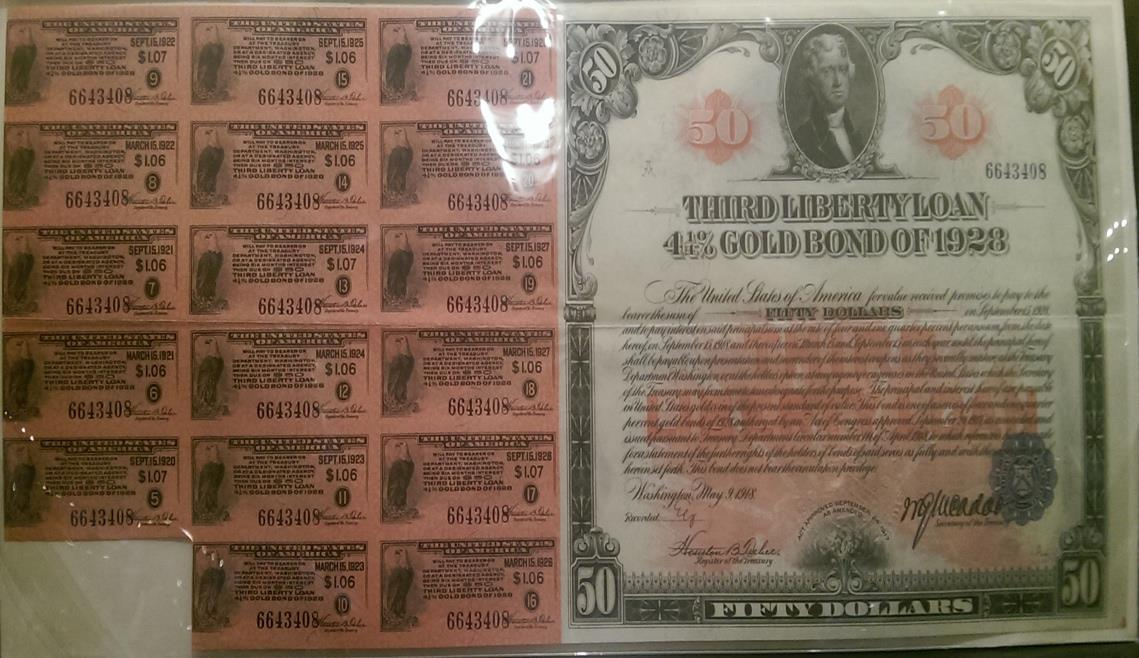
\includegraphics[width=1\linewidth]{pix_l3/Bondex.jpg}
\end{figure}
    
\end{column}
\begin{column}{0.48\textwidth}
\begin{itemize}
\item Issued: 1918
\item Due: 1928
\item Par: \$50
\item Rate: 4.25\%
\item Semi-annual
\item Used to fund World War I
\end{itemize}
\end{column}

    \end{columns}
    
\end{frame}


\begin{frame}{Bond Trading}
Bond trading takes place over-the-counter (OTC), a dealer market. The number of bond
issues far exceeds the number of stock issues (companies can have a dozen different bonds
and one stock), bond trades are much larger in size, and trades are less frequent than
stock.

\vspace{0.7em}
Lack of transparency: since 2002 dealers have to report trades and sale prices through
TRACE (Trade Reporting and Compliance Engine). Still if there are few trades or no trades
prices are not transparent.
\end{frame}

\subsection{Bond Pricing}
\begin{frame}{Bond Pricing}
The price of a bond is the present value of all cash flows generated by the bond (i.e.,
coupons and face value) discounted at the required rate of return.
\vspace{0.5cm}
$$P_B = \frac{CPN_1}{(1+r)^1} + \frac{CPN_2}{(1+r)^2} + \cdots + \frac{CPN_N}{(1+r)^N} + \frac{PAR}{(1+r)^N}$$
\vspace{0.5cm}
$$P_B = \frac{CPN}{r} \times \left[1 - \frac{1}{(1+r)^N}\right] + \frac{PAR}{(1+r)^N} \quad (2)$$
\end{frame}


\begin{frame}{Bond Pricing: Example 1}
What is the price of a 7.25\% annual coupon bond, with a \$1,000 face value, which matures
in 3 years? Assume a required return of 0.35\% and the time now is May 2013.
\vspace{0.5cm}
$$P_B = \frac{72.5}{0.0035} \times \left[1 - \frac{1}{(1 + 0.0035)^3}\right] + \frac{1000}{(1.0035)^3}$$
\vspace{0.5cm}
$$P_B = \$\LExOnePrice$$
\end{frame}


\begin{frame}{Example 1: Semi-annual Coupons}
What is the price of the bond if the coupons are paid semi-annually?
\vspace{0.5cm}
$$P_B = \frac{36.25}{0.00175} \times \left[1 - \frac{1}{(1 + 0.00175)^6}\right] + \frac{1000}{(1.00175)^6}$$
\vspace{0.5cm}
$$P_B = \$\LExOnePriceSemi$$
\end{frame}



\begin{frame}{Timeline of Bond Cash Flows}
\textbf{Annual coupon payments}
\vspace{0.1cm}
\begin{center}
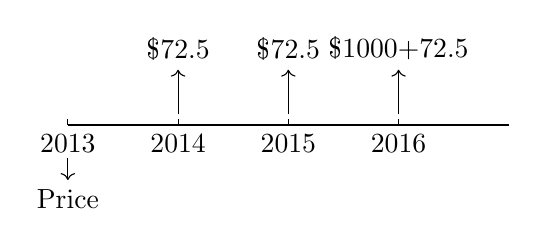
\begin{tikzpicture}[scale=0.7]
% Timeline
\draw[thick] (0,0) -- (8,0);
% Years
\foreach \x/\year in {0/2013, 2/2014, 4/2015, 6/2016}
{
  \draw (\x,0.1) -- (\x,0) node[below] {\year};
}
% Cash flows
\draw[->] (2,0.2) -- (2,1) node[above] {\$72.5};
\draw[->] (4,0.2) -- (4,1) node[above] {\$72.5};
\draw[->] (6,0.2) -- (6,1) node[above] {\$1000+72.5};
% Price arrow
\draw[->] (0,-0.6) -- (0,-1) node[below] {Price};
\end{tikzpicture}
\end{center}

\textbf{Semi-annual coupon payments}
\vspace{0.1cm}
\begin{center}
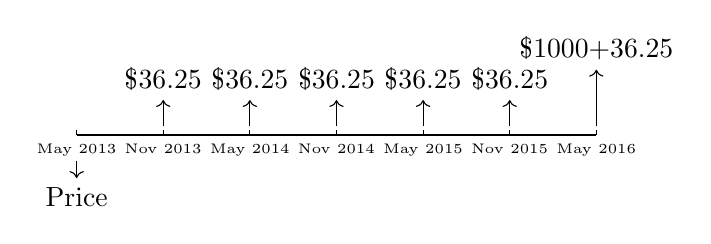
\begin{tikzpicture}[scale=0.55]
% Timeline
\draw[thick] (0,0) -- (12,0);
% Dates
\foreach \x/\date in {0/May 2013, 2/Nov 2013, 4/May 2014, 6/Nov 2014, 8/May 2015, 10/Nov 2015, 12/May 2016}
{
  \draw (\x,0.1) -- (\x,0) node[below] {\tiny\date};
}
% Cash flows
\foreach \x in {2,4,6,8,10}
{
  \draw[->] (\x,0.2) -- (\x,0.8) node[above] {\$36.25};
}
\draw[->] (12,0.2) -- (12,1.5) node[above] {\$1000+36.25};
% Price arrow
\draw[->] (0,-0.6) -- (0,-1) node[below] {Price};
\end{tikzpicture}
\end{center}


\end{frame}



\subsection{Bond Price and Yield to Maturity}
\begin{frame}{Yield to Maturity}
\keypoint{The yield to maturity (YTM) of a bond is the discount rate that sets the present
value of the promised bond payments equal to the current market price of the bond.}

YTM = y = r = IRR = required rate of return. YTM moves in line with the market interest
rate.
\end{frame}


\begin{frame}{Calculating YTM of a Bond: Example 2}
A five-year, \$1000 bond with 5\% coupon rate and semi-annual coupons is currently trading for a price of \$957.35. What is the bond's YTM?

\textbf{\underline{Solution}}
$$\$957.35 = \frac{\$25}{YTM} \times \left[1 - \frac{1}{(1 + YTM)^{10}}\right] + \frac{\$1000}{(1 + YTM)^{10}}$$

\textbf{By trial-and-error:}
\begin{itemize}
\item When YTM = Coupon rate = 2.5\%: Price = \$\LExTwoAtCoupon
\item Try YTM = 3.5\%: Price = \$\LExTwoAtHigh
\item Interpolation: $\frac{(YTM - 0.025)}{(0.035-0.025)} = \frac{(\LExTwoAtCoupon - \LExTwoPrice)}{(\LExTwoAtCoupon - \LExTwoAtHigh)}$
\item YTM $\approx$ \LExTwoYTM\%. The price function is convex, so interpolating between two trial rates overstates the yield slightly; solving exactly gives \LExTwoSemi\%, a \LExTwoAPR\% APR (\LExTwoSemi\% $\times$ 2)
\end{itemize}

By Excel: = rate(nper , pmt , pv , fv) = rate(10, 25, -\LExTwoPrice, 1000) = \LExTwoSemi\%
\end{frame}


\begin{frame}{A Bond's Price and Its YTM}
\keypoint{As bond yields rise, bond prices will fall, and vice versa.}

Because we can convert any price into a yield, and vice versa, prices and yields are used
interchangeably. Indeed, bond traders generally quote bond yields rather than prices.
\end{frame}


\subsection{Time and Interest Rate Effects}
\begin{frame}{Dynamic Behaviour of Bond Prices}
Coupon bonds may trade at prices lower, higher or the same as their face values because of
the effects of time and interest rates.

\vspace{0.8em}
\begin{center}
% Where a coupon bond trades relative to par, and the YTM-against-coupon-rate condition
% that puts it there. Replaces the three bullets that stated the same three cases.
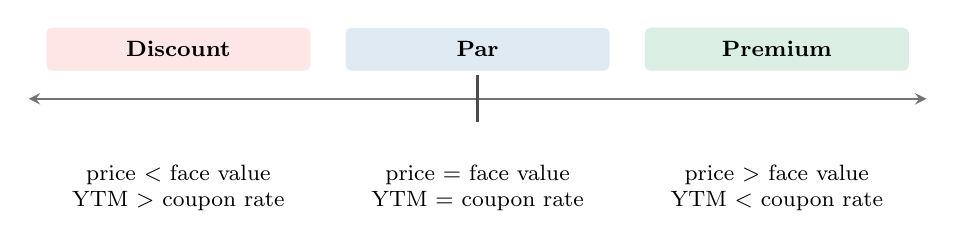
\begin{tikzpicture}[font=\footnotesize,>=stealth,
  band/.style={rounded corners=2pt,inner sep=5pt,text width=3.0cm,align=center},
  cond/.style={anchor=north,align=center,text width=3.4cm}]
\draw[<->,black!55,line width=0.8pt] (-0.2,0) -- (11.2,0);
\draw[black!70,line width=0.9pt] (5.5,0.3) -- (5.5,-0.3);

\node[band,fill=StAndrewsRed!12,anchor=south] at (1.7,0.35) {\textbf{Discount}};
\node[band,fill=StAndrewsBlue!12,anchor=south] at (5.5,0.35) {\textbf{Par}};
\node[band,fill=StAndrewsMidGreen!14,anchor=south] at (9.3,0.35) {\textbf{Premium}};

\node[cond] at (1.7,-0.72) {price $<$ face value\\ YTM $>$ coupon rate};
\node[cond] at (5.5,-0.72) {price $=$ face value\\ YTM $=$ coupon rate};
\node[cond] at (9.3,-0.72) {price $>$ face value\\ YTM $<$ coupon rate};
\end{tikzpicture}

\end{center}

\vspace{0.8em}
Zero-coupon bonds always trade at a discount: investors receive a face value which is
higher than the price paid for the bond.
\end{frame}


\begin{frame}{Time and Bond Prices: Zero-coupon Bonds}
Suppose you purchase a 30-year, zero-coupon bond with a YTM of 5\% and a face value of
\$100. What is the price of this bond five years later if the bond's YTM remains at 5\%?

\vspace{1em}
\begin{columns}[t]
\begin{column}{0.47\textwidth}
\keypoint{\centering The bond will initially trade for\\[4pt]{\Large\textbf{\$\LZeroInitial}}}
\end{column}
\begin{column}{0.47\textwidth}
\keypoint{\centering Five years later\\[4pt]{\Large\textbf{\$\LZeroLater}}}
\end{column}
\end{columns}

\vspace{1em}
\textit{The bond price is higher not because of the lower yield but less time to maturity}
\end{frame}


\begin{frame}{Time and Bond Prices: Coupon Bonds}
\keypoint{Bond prices rise as the next coupon payment gets closer and then drop after it
has been paid.}

This result also holds for coupon bonds. The pattern of price changes over time is
slightly more complicated because as time passes most of the cash flows get closer but
some disappear as the coupons get paid.
\end{frame}


\begin{frame}{The Effect of Time on Bond Prices: Example 3}
Consider a 30-year bond with a 10\% coupon rate (annual payments) and a face value of
\$100.
\vfill
1. What is the initial price of this bond if it has a 5\% YTM?\\
2. If the YTM is unchanged, what will the price be immediately BEFORE and AFTER the first
coupon is paid?
\vfill
\end{frame}


\begin{frame}{Example 3: Solution}
\vspace{0.5cm}
\begin{align}\nonumber
P_{Initial} &= \frac{10}{0.05} \times \left[1 - \frac{1}{1.05^{30}}\right] + \frac{100}{1.05^{30}} = \$\LExThreeInitial \\[8pt]\nonumber
P_{Before} &= 10 + \frac{10}{0.05} \times \left[1 - \frac{1}{1.05^{29}}\right] + \frac{100}{1.05^{29}} = \$\LExThreeBefore \\[8pt]\nonumber
P_{After} &= \frac{10}{0.05} \times \left[1 - \frac{1}{1.05^{29}}\right] + \frac{100}{1.05^{29}} = \$\LExThreeAfter
\end{align}
\end{frame}



\begin{frame}{Example 3: Some Discussions}
\vspace{0.4em}
\begin{terms}
Immediately BEFORE the coupon payment & The bond price is higher than the initial price: no
  changes in the number of coupon payments but an investor does not have to wait as long to
  receive the first coupon payment. \\
Immediately AFTER the coupon payment & The bond price drops by the amount of the coupon
  (\$10): the new bond owner will not receive this first coupon payment. \\
After the first payment & The price becomes lower than the initial price: fewer coupon
  payments remaining, investors pay less for the bond. \\
\end{terms}
\end{frame}


\begin{frame}{Time and Bond Prices: Graphical Presentation}
\begin{center}
% Four 30-year bonds at a 5% YTM. Between coupons the price grows at the yield and
% on a coupon date it drops by the coupon, which is what makes the sawtooth.
\begin{tikzpicture}
\begin{axis}[lectureplot,width=10.4cm,height=5.4cm,xmin=0,xmax=35,ymin=0,ymax=232,
xtick={0,5,10,15,20,25,30,35},ytick={0,20,40,60,80,100,120,140,160,180,200},
xlabel={Year},ylabel={Bond price (\$)},
every axis plot/.append style={line width=0.7pt,no marks}]
\addplot[StAndrewsMidBlue] table[x=year,y=price]{generated/time_ten.dat};
\addplot[StAndrewsRed]     table[x=year,y=price]{generated/time_five.dat};
\addplot[StAndrewsGreen]   table[x=year,y=price]{generated/time_two.dat};
\addplot[StAndrewsPurple]  table[x=year,y=price]{generated/time_zero.dat};
\node[anchor=west,font=\footnotesize,text=StAndrewsMidBlue] at (axis cs:2.5,158) {10\% coupon rate};
\node[anchor=west,font=\footnotesize,text=StAndrewsRed]     at (axis cs:2.5,88)  {5\% coupon rate};
\node[anchor=west,font=\footnotesize,text=StAndrewsGreen]   at (axis cs:2.5,44)  {2\% coupon rate};
\node[anchor=west,font=\footnotesize,text=StAndrewsPurple]  at (axis cs:2.5,14)  {0\% coupon rate};
\node[draw=StAndrewsRed,line width=0.6pt,anchor=north east,align=left,font=\footnotesize,
      inner sep=4pt] at (axis cs:35,230)
      {YTM: 5\%\\Maturity: 30 years\\Par: \$100};
\end{axis}\end{tikzpicture}

\end{center}
\end{frame}


\begin{frame}{Interest Rate Changes and Bond Prices}
\keypoint{When interest rates rise, investors demand high yields (higher discount rates),
reducing the price of bonds.}

As interest rates in the economy fluctuate, the yield that investors demand from bonds
will also change, as do the bond prices.
\end{frame}


\begin{frame}{The Interest Rate Sensitivity of Bond Prices}
\vspace{0.8em}
\begin{center}
\resizebox{\linewidth}{!}{% Two ways a bond price becomes more sensitive to interest rates. The arrows draw the
% two sentences the slide used to spell out twice in words.
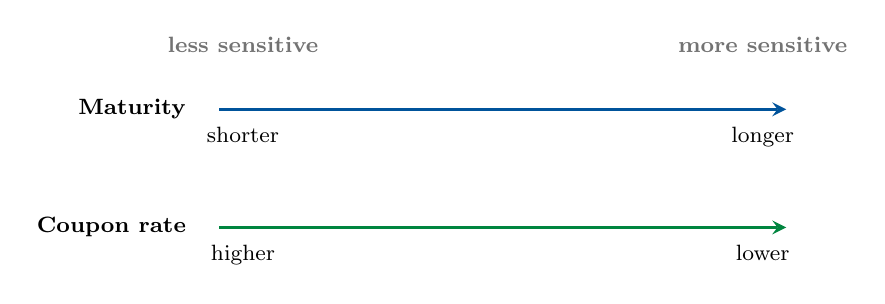
\begin{tikzpicture}[font=\footnotesize,>=stealth]
\node[anchor=south,black!55] at (3.2,2.6) {\textbf{less sensitive}};
\node[anchor=south,black!55] at (9.8,2.6) {\textbf{more sensitive}};

\node[anchor=east] at (2.6,2.0) {\textbf{Maturity}};
\draw[->,StAndrewsBlue,line width=1.2pt] (2.9,2.0) -- (10.1,2.0);
\node[anchor=north,inner sep=4pt] at (3.2,1.92) {shorter};
\node[anchor=north,inner sep=4pt] at (9.8,1.92) {longer};

\node[anchor=east] at (2.6,0.5) {\textbf{Coupon rate}};
\draw[->,StAndrewsMidGreen,line width=1.2pt] (2.9,0.5) -- (10.1,0.5);
\node[anchor=north,inner sep=4pt] at (3.2,0.42) {higher};
\node[anchor=north,inner sep=4pt] at (9.8,0.42) {lower};
\end{tikzpicture}
}
\end{center}
\end{frame}


\begin{frame}{Sensitivity of Bond Prices to Interest Rate}
\framesubtitle{Different Maturities}
\begin{center}
% A five-year and a thirty-year bond, both 10% coupon, priced across the required
% return. The annotations are the price change over each five-point step.
\begin{tikzpicture}
\begin{axis}[sensitivityplot]
\addplot[StAndrewsMidGreen] table[x=rate,y=price]{generated/rate_thirty_year.dat};
\addplot[StAndrewsRed]      table[x=rate,y=price]{generated/rate_five_year.dat};
\node[anchor=west,font=\footnotesize,text=StAndrewsRed]      at (axis cs:25.4,60) {5-year bond};
\node[anchor=west,font=\footnotesize,text=StAndrewsMidGreen] at (axis cs:25.4,40) {30-year bond};
\node[draw=StAndrewsRed,line width=0.6pt,anchor=south west,align=left,font=\footnotesize,
      inner sep=4pt] at (axis cs:0.6,12) {Par: \$100\\Coupon rate: 10\%};
\node[anchor=north west,align=center,font=\footnotesize,text=StAndrewsMidGreen]
      at (axis cs:14,198) {\underline{30-year}\\\LThirtyA\%\\\LThirtyB\%\\\LThirtyC\%\\\LThirtyD\%};
\node[anchor=north west,align=center,font=\footnotesize,text=StAndrewsRed]
      at (axis cs:21,198) {\underline{5-year}\\\LFiveYrA\%\\\LFiveYrB\%\\\LFiveYrC\%\\\LFiveYrD\%};
\end{axis}\end{tikzpicture}

\end{center}
\end{frame}


\begin{frame}{Sensitivity of Bond Prices to Interest Rate}
\framesubtitle{Different Coupon Rates}
\begin{center}
% Two fifteen-year bonds, 1% and 10% coupon, priced across the required return.
\begin{tikzpicture}
\begin{axis}[sensitivityplot,ymax=160,ytick={0,20,40,60,80,100,120,140,160}]
\addplot[StAndrewsBlue]   table[x=rate,y=price]{generated/coupon_ten_percent.dat};
\addplot[StAndrewsOrange] table[x=rate,y=price]{generated/coupon_one_percent.dat};
\node[anchor=west,font=\footnotesize,text=StAndrewsBlue] at (axis cs:25.4,42)
      {10-percent coupon rate};
\node[anchor=west,font=\footnotesize,text=StAndrewsOrange] at (axis cs:25.4,8)
      {1-percent coupon rate};
\node[draw=StAndrewsRed,line width=0.6pt,anchor=west,align=left,font=\footnotesize,
      inner sep=4pt] at (axis cs:1.2,19) {Par: \$100\\Maturity: 15 years};
\node[anchor=north west,align=center,font=\footnotesize,text=StAndrewsBlue]
      at (axis cs:18.4,158) {\underline{10-percent}\\\LCouponTenA\%\\\LCouponTenB\%\\\LCouponTenC\%\\\LCouponTenD\%};
\node[anchor=north west,align=center,font=\footnotesize,text=StAndrewsOrange]
      at (axis cs:24.4,158) {\underline{1-percent}\\\LCouponOneA\%\\\LCouponOneB\%\\\LCouponOneC\%\\\LCouponOneD\%};
\end{axis}\end{tikzpicture}

\end{center}
\end{frame}


\begin{frame}{Sensitivity of Bond Prices: Time and Interest Rate}
In actuality, bond prices are subject to both time effect and interest rate changes.

\vspace{0.9em}
\begin{terms}
Time effect & Bond prices converge to the bond's face value. \\
Interest rate effect & Bond prices move up and down due to changes in bond yields. \\
\end{terms}
\end{frame}


\begin{frame}{Time and Interest Rate: Example 4}
Consider a \textcolor{StAndrewsBlue}{15-year zero-coupon bond} and a \textcolor{StAndrewsGreen}{30-year coupon bond with 10\% annual coupons} (\$100 face value). By what percentage will the price of each bond change if its YTM increases from 5\% to 6\%?

\end{frame}



\begin{frame}{Example 4: Solution}
\textbf{15-year zero-coupon bond}
\begin{align}\nonumber
P_{15,5\%} &= \frac{100}{1.05^{15}} = \$\LExFourZeroFive \\\nonumber
P_{15,6\%} &= \frac{100}{1.06^{15}} = \$\LExFourZeroSix \\\nonumber
\Delta P_{15} &= \frac{(\LExFourZeroSix-\LExFourZeroFive)}{\LExFourZeroFive} = \LExFourZeroChange\%
\end{align}

\textbf{30-year coupon bond}
\begin{align}\nonumber
P_{30,5\%} &= \frac{10}{0.05} \times \left[1 - \frac{1}{1.05^{30}}\right] + \frac{100}{1.05^{30}} = \$\LExFourCouponFive \\\nonumber
P_{30,6\%} &= \frac{10}{0.06} \times \left[1 - \frac{1}{1.06^{30}}\right] + \frac{100}{1.06^{30}} = \$\LExFourCouponSix \\\nonumber
\Delta P_{30} &= \frac{(\LExFourCouponSix-\LExFourCouponFive)}{\LExFourCouponFive} = \LExFourCouponChange\%
\end{align}
\end{frame}


\subsection{The Yield Curve}
\begin{frame}{The Yield Curve: Description}
\keypoint{A plot of relationship between bond YTM and time to maturity is known as the
yield curve.}

A yield curve can also be described as the term structure of interest rates.
\end{frame}


\begin{frame}{The Yield Curve: Graph}
\begin{center}
% Bank of England nominal government liability curve, one trading day.
\begin{tikzpicture}
\begin{axis}[lectureplot,width=10.4cm,height=5.2cm,xmin=0,xmax=40,
ymin=4,ymax=6,xtick={0,5,10,15,20,25,30,35,40},ytick={4,4.5,5,5.5,6},minor y tick num=1,
yticklabel={\pgfmathprintnumber[fixed,precision=1]{\tick}\%},
xlabel={Maturity (years)},ylabel={Yield to maturity}]
\addplot[StAndrewsLightBlue,line width=1pt,mark=*,mark size=1pt,
         mark options={fill=StAndrewsLightBlue,draw=none}]
        table[x=maturity,y=yield]{generated/yield_curve.dat};
\end{axis}\end{tikzpicture}


\tiny{Source: Bank of England nominal government liability curve, \LCurveDate\ \url{https://www.bankofengland.co.uk/statistics/yield-curves}}
\end{center}
\end{frame}


\subsection{Corporate Bonds and Risk of Default}
\begin{frame}{Corporate Bonds}
\keypoint{For corporate bonds, the issuer may default; this risk is known as credit risk.}

Government bonds tend to be safe in terms of default (at least those denominated in local
currency). Investors pay less for bonds with credit risk than they would for default-free
(additional yield = default premium).
\end{frame}


\begin{frame}{Risk of Default and Risk Premium}
\textbf{Example 5}

Andrew Corporation issues a one-year zero coupon bond with a face value of \$1000. Potential bondholders expect there to be a 50\% chance that the bond will repay its face value in full (if the economy becomes stronger) and a 50\% chance that the bond will default, and bondholders will receive only 90\% of the face value at the end of one year (if the economy becomes weaker). As a result, investors buy the bond for \$920. Assume that the one-year risk-free interest rate is 2\%.
\vfill
1. What is the expected and promised YTM of the bond?\\
2. What is the default risk premium required by investors for this bond?
\end{frame}


\begin{frame}{Example 5: Solution}
\begin{align}\nonumber
\text{Expected cash inflow} &= 0.5 \times 1000 + 0.5 \times 900 = \$\LExFivePayoff \\[4pt]\nonumber
\text{Expected YTM} &= (\LExFivePayoff / 920) - 1 = \LExFiveExpected\% \\[4pt]\nonumber
\text{Promised YTM} &= (1000 / 920) - 1 = \LExFivePromised\% \\[4pt]\nonumber
\text{Risk premium} &= \LExFiveExpected\% - 2\% = \LExFivePremium\%
\end{align}

\vspace{0.4em}
The \LExFivePromised\% promised YTM is the most investors will receive (no default). If the
company defaults, investors will receive only \$900, a return of
$(900 / 920) - 1 = -\LExFiveDefault\%$. The average return (the cost of debt) is
$\LExFiveExpected\% = 0.5 \times \LExFivePromised\% + 0.5 \times (-\LExFiveDefault\%)$.
\end{frame}

\begin{frame}{Bond Ratings}
The safety of most corporate bonds can be judged from bond ratings provided by Moody's,
Standard and Poor's, Fitch Ratings or other bond rating firms.

\vspace{0.6em}
\begin{terms}
Highest quality & Aaa (Moody's), AAA (S\&P, Fitch) \\
Investment-grade bonds & Baa, BBB and above \\
Speculative / junk / high-yield bonds & Below Baa \\
\end{terms}

\vspace{0.6em}
Protection against default risk: seniority, security and protective covenants
\begin{itemize}
\item Extra debt restriction
\item No senior new debt
\item Gearing limit
\end{itemize}
\end{frame}

\section{Stocks Valuation}



\begin{frame}{Topics Covered}
\begin{itemize}
\item Stocks and Stock Trading
\item Valuing Common Stocks
\item The Dividend Discount Model
\item Repurchases and the Total Payout Model
\item Valuation Based on Comparable Firms
\end{itemize}

\end{frame}

\begin{frame}{Reading}
\begin{itemize}
\item HRWJJ - Chapter 5
\item BMAE - Chapter 4 
\item Pinto, J.E., Robinson, T.R. and Stowe, J.D. (2019) Equity Valuation: A Survey of Professional Practice. \textit{Review of Financial Economics} 37, 219-233. \url{https://doi.org/10.1002/rfe.1040}
\item Brav, A., Graham, J.R., Harvey, C.R. and Michaely, R. (2005) Payout Policy in the 21st Century. \textit{Journal of Financial Economics} 77, 483-527. \url{https://doi.org/10.1016/j.jfineco.2004.07.004}
\end{itemize}

\end{frame}


\subsection{Stocks and Stock Trading}
\begin{frame}{Common Stock}
\vspace{0.5em}
\begin{terms}
Common stock & A certificate of capital ownership in a publicly held corporation. \\
Dividend & Periodic cash distribution from the firm to the shareholders. \\
Capital gain & Earnings come from selling stocks. \\
\end{terms}
\end{frame}


\begin{frame}{Classes of Common Stocks}
\vspace{0.5em}
A primary reasons for firms creating multiple classes of stock is to do with control of
the firm. Firms can raise equity capital by issuing nonvoting or limited-voting stock.
\end{frame}


\begin{frame}{Berkshire Hathaway}
    
\begin{columns}
    
\begin{column}{0.48\textwidth}

            \begin{figure}
    \centering
    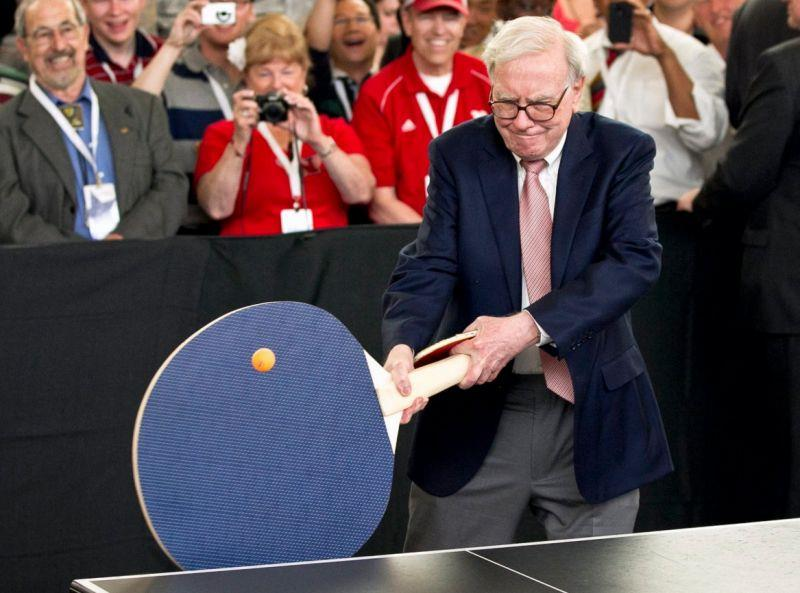
\includegraphics[width=1\linewidth]{pix_l3/berkshire.jpg}
\end{figure}
    
\end{column}
\begin{column}{0.48\textwidth}
\begin{itemize}
\item Class B (BRK.B) shares have 1/10,000\textsuperscript{th} of the voting rights of Class A (BRK.A) shares
\item B shares have value 1/1,500\textsuperscript{th} of Class A shares
\end{itemize}
\end{column}

    \end{columns}


\end{frame}


\begin{frame}{Ford, General Motors, Alphabet (Google)}
\vspace{0.5em}
\begin{terms}
Ford & Class B represents less than 10\% of the number of shares outstanding but has 40\%
  voting power. \\
GM & Class E is to partly finance acquisition of Electronic Data Systems (1984) and class H
  for Hughes Aircraft (1985). \\
Alphabet (Google) & Class C (GOOG) has no voting rights; class A (GOOGL) has one vote each;
  class B has ten votes each (which do not trade in the public market). \\
\end{terms}
\end{frame}



\begin{frame}{Stock Trading – Organised Stock Exchange}
\vspace{0.4em}
\begin{terms}
Over-the-counter & Market participants look up the prices quoted and trade with dealers
  (dealer market). \\
Electronic trading system & Market participants post orders over computer networks and
  trading is done automatically without human intervention when orders are matched
  ('crossed'). \\
\end{terms}

\vspace{0.8em}
Brokers, Dealers and Designated Market Makers (Specialists). Highly regulated.
\end{frame}


\begin{frame}{Stock Price Listings}
\begin{center}
% The summary quote a student would read off a stock listing. Figures come from
% data/hon_quote.csv, so the panel is typeset rather than screenshotted.
\begin{minipage}{0.86\textwidth}
{\large\textbf{Honeywell International Inc. (HON)}~{\color{black!55}NYSE}}\par
\vspace{2pt}
{\Large\textbf{\LHonPrice}}~{\color{StAndrewsMidGreen}\textbf{\LHonChange\ (\LHonChangePct\%)}}\par
\vspace{4pt}
{\color{black!55}\rule{\linewidth}{0.4pt}}\par
\vspace{4pt}
\footnotesize
\begin{tabular}{@{}l r@{\hspace{2.2em}}l r@{}}
Prev close       & \LHonPrevClose  & Day's range   & \LHonDayLow--\LHonDayHigh \\
Open             & \LHonOpen       & 52wk range    & \LHonYearLow--\LHonYearHigh \\
Volume           & \LHonVolume     & Market cap    & \LHonMarketCap bn \\
Avg vol (3m)     & \LHonAvgVolume  & P/E (ttm)     & \LHonPE \\
Beta             & \LHonBeta       & EPS (ttm)     & \LHonEPS \\
                 &                 & Div \& yield  & \LHonDividend\ (\LHonDividendYield\%) \\
\end{tabular}
\end{minipage}


\vspace{0.3cm}
\tiny{Source: \url{https://uk.finance.yahoo.com} [\LHonAsOf]}
\end{center}
\end{frame}


\begin{frame}{Types of Orders}
\vspace{0.5em}
\begin{terms}
Limit orders & An order to buy or sell shares at a predetermined price, to be executed
  when the market price reaches the requested price. \\
Market orders & An order to buy or sell shares at the best currently available market
  price. \\
\end{terms}
\end{frame}


\begin{frame}{Types of Limit Orders}
\begin{center}
% The four limit orders placed around today's price: two fire when the price rises, two
% when it falls. Replaces the six bullets that described the same four orders.
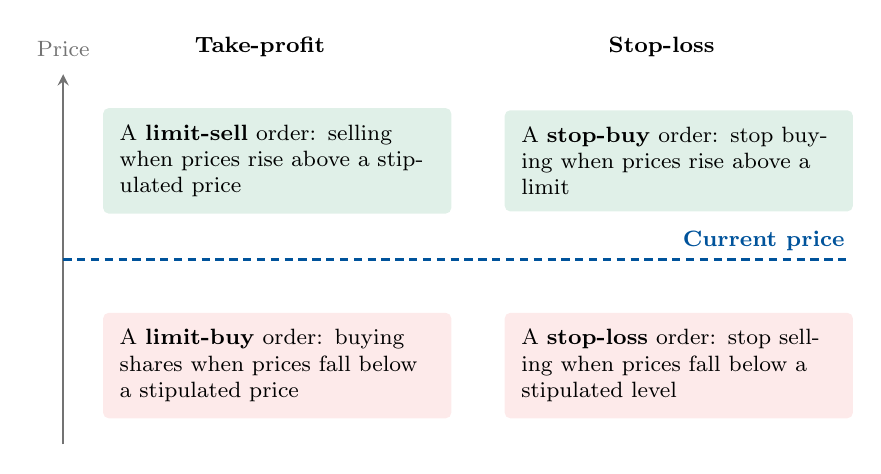
\begin{tikzpicture}[font=\footnotesize,>=stealth,
  order/.style={rounded corners=2pt,inner sep=6pt,text width=4.0cm,align=left}]
\draw[->,black!55,line width=0.8pt] (0,-2.35) -- (0,2.35);
\node[anchor=south,black!55] at (0,2.45) {Price};
\node[anchor=south] at (2.5,2.45) {\textbf{Take-profit}};
\node[anchor=south] at (7.6,2.45) {\textbf{Stop-loss}};

\node[order,fill=StAndrewsMidGreen!12,anchor=west] at (0.5,1.25)
  {A \textbf{limit-sell} order: selling when prices rise above a stipulated price};
\node[order,fill=StAndrewsMidGreen!12,anchor=west] at (5.6,1.25)
  {A \textbf{stop-buy} order: stop buying when prices rise above a limit};

\draw[StAndrewsBlue,line width=1pt,dash pattern=on 3pt off 2pt] (0,0) -- (10.0,0);
\node[anchor=south east,StAndrewsBlue,inner sep=2pt] at (10.0,0.03) {\textbf{Current price}};

\node[order,fill=StAndrewsRed!10,anchor=west] at (0.5,-1.35)
  {A \textbf{limit-buy} order: buying shares when prices fall below a stipulated price};
\node[order,fill=StAndrewsRed!10,anchor=west] at (5.6,-1.35)
  {A \textbf{stop-loss} order: stop selling when prices fall below a stipulated level};
\end{tikzpicture}

\end{center}
\end{frame}

\subsection{Valuing Common Stocks}
\begin{frame}{Common Stock Valuation}
\keypoint{The value of a stock is the present value of its current and expected future
cash flows.}

A common stock is more difficult to value in practice than a bond:
\begin{itemize}
\item Promised cash flows are unknown in advance
\item Common stocks have no maturity
\item The rate of return that the market requires is unobservable
\end{itemize}
\end{frame}


\begin{frame}{Stock Prices: One-year Investment Horizon}
Two potential sources of cash flows from owning a stock:
\begin{itemize}
\item Dividend
\item Capital gain
\end{itemize}

\vspace{0.5cm}
Assuming for simplicity that an investor buys a stock today and sells it at the end of the
year and all dividends are also paid at the end of the year.

\vspace{0.5cm}
\begin{center}
\boxed{P_{0(1)} = \frac{D_1 + P_1}{(1+r_e)} \quad (1)}
\end{center}
\end{frame}


\begin{frame}{Dividend Yields and Capital Gains}
Eq.(1) can be transformed into (2):

\vspace{0.5cm}
\begin{center}
\boxed{r_e = \frac{D_1}{P_0} + \frac{P_1-P_0}{P_0} \quad (2)}
\end{center}

\vspace{0.5cm}
\begin{itemize}
\item The first term on the right-hand side is the dividend yield and the second term is the capital gain rate
\item The sum is the total return of the stock
\item If the stock offered a higher return than other securities with the same risk, investors would sell other investments and buy the stock, driving up the current price of the stock
\end{itemize}
\end{frame}

\begin{frame}
\frametitle{A 2-year Investor}
Suppose an investor planned to hold the stock for two years, then this investor would
receive dividends in both year 1 and year 2 before selling the stock. Setting the stock
price equal to the present value of the future cash flows in this case implies:

\vspace{1cm}
\begin{center}
\boxed{P_{0(2)} = \frac{D_1}{(1+r_e)} + \frac{(D_2+P_2)}{(1+r_e)^2} \quad (3)}
\end{center}
\end{frame}


\subsection{The Dividend Discount Model}
\begin{frame}{Dividend-Discount Model (DDM)}
We can continue this process for any number of years by replacing the final price with the
value that the next holder of the stock would be willing to pay. Doing so leads to the
general dividend-discount model:

\vspace{0.5cm}
\begin{center}
\boxed{P_{0,N} = \frac{D_1}{(1+r_e)} + \frac{D_2}{(1+r_e)^2} + \cdots + \frac{D_N+P_N}{(1+r_e)^N} \quad (4)}
\end{center}

\vspace{0.5cm}
If it is possible to hold the stock forever, we can let N go to infinity:

\begin{center}
\boxed{P_{0,N} = \frac{D_1}{(1 + r_e)} + \frac{D_2}{(1 + r_e)^2} + \cdots = \sum_{n=1}^{\infty} \frac{D_n}{(1 + r_e)^n} \quad (5)}
\end{center}
\end{frame}

\begin{frame}{Case 1: Zero Growth}
For a zero growth common stock, the dividend is constant through time:
$$D_1 = D_2 = D_3 = \text{constant}$$

So the value of the stock is:
$$P_0 = \frac{D}{(1+r)} + \frac{D}{(1+r)^2} + \frac{D}{(1+r)^3} + \cdots$$

The stock can be viewed as an ordinary perpetuity, and the per-share value is thus given
by:

\vspace{0.2cm}
\begin{center}
\boxed{P_0 = \frac{D}{r} \quad (6)}
\end{center}
\end{frame}

\begin{frame}{Case 2: Constant Growth DDM}
Another simplification of the DDM is to assume that dividends grow at a constant rate
(Gordon Growth Model):

\begin{align}\nonumber
D_1 &= D_0(1 + g) \\[2pt]\nonumber
D_2 &= D_1(1 + g) = D_0(1 + g)^2 \\[2pt]\nonumber
D_3 &= D_2(1 + g) = D_0(1 + g)^3
\end{align}

$$P_0 = \frac{D_1}{(1+r)} + \frac{D_1(1+g)}{(1+r)^2} + \frac{D_1(1+g)^2}{(1+r)^3} + \cdots$$
\vspace{0.2cm}
\begin{center}
\boxed{P_0 = \frac{D_1}{(r - g)} = \frac{D_0(1 + g)}{(r - g)} \quad (7)}
\end{center}
\end{frame}

% Slide 10: Constant Growth: Example 1
\begin{frame}{Constant Growth: Example 1}
\textbf{Example 1}

Suppose Edison Company plans to pay £2.30 per share in dividends in the coming year. If the required rate of return is 7\% and dividends are expected to grow by 2\% per year in the future, how much should Edison's stock be selling for?

\vspace{1cm}
\textbf{Solution}
\begin{align}\nonumber
P_0 &= \frac{D_1}{(r - g)} \\\nonumber
&= \frac{2.30}{(0.07 - 0.02)} \\\nonumber
&= \text{\pounds}\LEdisonPrice
\end{align}


\end{frame}

\begin{frame}{Constant Growth: Example 2}
\textbf{Example 2}

Suppose Blue Skies Company just paid a dividend of £0.50 per share. It is expected to increase its dividend by 2\% per year. If the market requires a return of 15\% on assets of a similar risk level taken by the company, how much should the stock be selling for?

\vspace{1cm}
\textbf{Solution}
\begin{align}\nonumber
P_0 &= \frac{D_0(1 + g)}{(r - g)} \\\nonumber
&= \frac{0.50(1 + 0.02)}{(0.15 - 0.02)} \\\nonumber
&= \text{\pounds}\LBlueSkiesPrice
\end{align}


\end{frame}

\begin{frame}{Constant Growth: Example 3}
\textbf{Example 3}

Suppose Gordon Company will pay a dividend of £4 per share in the coming year. Investors require a 16\% return on companies such as Gordon. Gordon's dividend is expected to increase by 6\% every year. What is the value of Gordon's stock today? What is the value in four years?

\vspace{0.5cm}
\textbf{Solution}
\begin{align}\nonumber
P_0 &= \frac{D_1}{(r - g)} = \frac{4}{(0.16 - 0.06)} = \text{\pounds}\LGordonPrice \\\nonumber
P_4 &= \frac{D_5}{(r-g)} = \frac{D_1(1+g)^4}{(r-g)} = \frac{4(1+0.06)^4}{(0.16-0.06)} = \text{\pounds}\LGordonPriceFour \\\nonumber
P_4 &= P_0(1 + g)^4 = \LGordonPrice(1 + 0.06)^4 = \text{\pounds}\LGordonPriceFour
\end{align}

Stock price will grow at the same constant rate as dividend.

\end{frame}


\begin{frame}{Dividends vs. Investment and Growth}
To maximise its share price, a firm would like to increase both the dividend level and
expected growth rate as shown in Eq.(7).

\vspace{0.9em}
\begin{center}
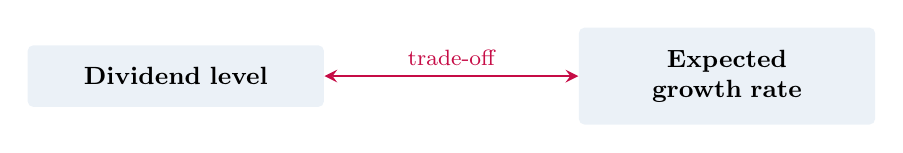
\begin{tikzpicture}[font=\small,>=stealth]
\node[fill=StAndrewsBlue!8,rounded corners=2pt,inner sep=8pt,text width=3.2cm,
      align=center] (d) at (0,0) {\textbf{Dividend level}};
\node[fill=StAndrewsBlue!8,rounded corners=2pt,inner sep=8pt,text width=3.2cm,
      align=center] (g) at (7,0) {\textbf{Expected growth rate}};
\draw[<->,StAndrewsBurgundy,line width=1pt] (d.east) --
  node[above,font=\footnotesize] {trade-off} (g.west);
\end{tikzpicture}
\end{center}

\vspace{0.6em}
However, there is often a trade-off: growth requires investment, which reduces dividend
payout. The constant growth model will help to gain insight into this trade-off.
\end{frame}


\begin{frame}{Dividend Payout}
If the dividend payout rate (DPR) is defined as the fraction of a firm's earnings that the
firms pay as dividends each year, the firm's dividend per share at date $t$ is as follows:

\begin{center}
\boxed{D_t = \frac{\text{Earnings}_t}{\text{Shares outstanding}_t} \times \text{DPR}_t = \text{EPS}_t \times \text{DPR}_t \quad (8)}
\end{center}

\vspace{0.6em}
The firm can increase dividend in 3 ways:
\begin{enumerate}
\item By increasing its earnings
\item By increasing its dividend payout rate
\item By reducing its shares outstanding
\end{enumerate}
\end{frame}


\begin{frame}{A Simple Model of Growth}
To explore the trade-off between growth in earnings (1) and dividend (2), let's suppose
that the number of shares outstanding (3) is fixed.

\begin{align}\nonumber
\Delta\text{Earnings}_{(t,t+1)} &= \text{Invest.}_{(t+1)} \times \text{Return on Invest.}_{(t+1)} \quad (9) \\\nonumber
\text{Invest.}_{(t+1)} &= \text{Retained Earnings}_t \\\nonumber
\text{Retained Earnings}_t &= \text{Earnings}_t \times \text{Retention Rate}_t \quad (10) \\\nonumber
\text{Earnings Growth}_{(t,t+1)} =g &= \frac{\Delta\text{Earnings}_{(t,t+1)}}{\text{Earnings}_t} \\\nonumber
g &= \text{Retention Rate}_t \times \text{Return on Invest.}_{(t+1)} \quad (11)
\end{align}
\end{frame}

\begin{frame}{Profitable Growth}
Eq. (11) shows that a firm can increase its growth rate by retaining more earnings.
However, the firm will have to reduce its dividend, as shown in Eq. (8).

\vspace{1em}
If a firm wants to increase its share price, should it\ldots

\vspace{0.6em}
\begin{columns}[c]
\begin{column}{0.44\textwidth}
\keypoint{\centering cut dividend and invest more?}
\end{column}
\begin{column}{0.06\textwidth}
\centering\textit{or}
\end{column}
\begin{column}{0.44\textwidth}
\keypoint{\centering cut investment and increase its dividend?}
\end{column}
\end{columns}
\end{frame}


\begin{frame}{Cutting Dividends for Profitable Growth}
\textbf{Example 4}

Sports Wear expects to have earnings per share of €7 in the coming year. Rather than reinvest these earnings and grow, the firm plans to pay out all of its earnings as a dividend. With these expectations of no growth (assuming that Sports Wear does not buy back shares and raises funds for investment by issuing more shares or increasing debt), the firm's current stock price is €55.

Suppose Sports Wear could cut its dividend payout rate to 70\% for the foreseeable future and use the retained earnings to open new stores. The return on its investment in these new stores is expected to be 15\%. Assuming the required rate of return from investors is unchanged, what would the current stock price be?

\end{frame}



% Slide 16: Example 4: Solution
\begin{frame}{Example 4: Solution}
First, estimate the required rate of return (the firm's cost of capital):
\begin{align}\nonumber
r_e &= \frac{D_1}{P_0} + g = \frac{7}{55} + 0\% = \LSportsRequired\%
\end{align}

If the firm reduces its DPR to 70\%, then:
\begin{align}\nonumber
D_1 &= 7 \times 70\% = \LSportsDividend \\\nonumber
g &= (1 - 70\%) \times 15\% = \LSportsGrowth\% \\\nonumber
P_0 &= \frac{D_1}{r_e - g} = \frac{\LSportsDividend}{\LSportsRequired\% - \LSportsGrowth\%} = \text{€}\LSportsPrice > \text{€} 55
\end{align}

Cutting the firm's dividend in favour of growth raised the firm's stock price. But is this always the case?

\end{frame}

\begin{frame}{Example 5: Unprofitable Growth}
Suppose Sports Wear decides to cut its dividend payout rate to 70\% to invest in new stores as in Example 4 but now the return on this new investment is 10\% rather than 15\%. Given its expected earnings per share of €7 and its cost of capital of \LSportsRequired\%, what will happen to the firm's current share price in this case?

\vspace{1cm}
\textbf{Solution}
\begin{align}\nonumber
g &= (1 - 70\%) \times 10\% = \LSportsGrowthBad\% \\\nonumber
P_0 &= \frac{D_1}{r_e - g} = \frac{\LSportsDividend}{\LSportsRequired\% - \LSportsGrowthBad\%} = \text{€}\LSportsPriceBad < \text{€} 55
\end{align}

The new investment has negative NPV: return on new investment < return required by investors, so the share price will fall if the firm cuts its dividend to make this new investment


\end{frame}

% Slide 17: Profitable vs. Unprofitable Growth
\begin{frame}{Profitable vs. Unprofitable Growth}
\keypoint{Cutting the firm's dividend to increase investment will raise the stock price
if, and only if, the return on new investment exceeds the return required by investors.}

The effect of cutting dividend to grow crucially depends on the return on new investment.
If new investment is expected to earn only the return required by investors, reinvesting
earnings does not add value to stock price (even though it will lead to earnings growth).
\end{frame}

\begin{frame}
\frametitle{Growth and Business Life Cycle}
\vspace{0.6em}
\begin{columns}[t]
\begin{column}{0.47\textwidth}
\textbf{Successful young firms} often have very high earnings growth rates; these firms
tend to retain all earnings for investment.
\end{column}
\begin{column}{0.47\textwidth}
\textbf{As they mature,} these firms grow slower, earnings exceed their investment needs
and they begin to pay dividends.
\end{column}
\end{columns}

\vspace{1.2em}
The constant growth DDM cannot be used.
\end{frame}


\begin{frame}{Case 3: Differential Growth}
However, we can use the general form of the DDM to value these firms. Assume that
dividends will grow at a certain rate in the foreseeable future ($g_1$) and then grow at a
different rate ($g_2$) thereafter.

\vspace{0.8em}
To value a differential growth stock:
\begin{enumerate}
\item Estimate the future dividends in the foreseeable future and calculate the present value of these dividends (from year 1 to N)
\item Estimate the future stock price ($P_N$) when the stock becomes a constant growth stock
\item Calculate the total present value of (1) and (2)
\end{enumerate}
\end{frame}


\begin{frame}{Case 3: Differential Growth Timeline}
\begin{center}
% Dividends grow at g1 to date N, then at g2 forever. Redrawn from the raster the
% deck used to carry.
\begin{tikzpicture}[font=\footnotesize,>=stealth]
\draw[StAndrewsRed,line width=1pt] (0,0) -- (4.4,0);
\draw[StAndrewsRed,line width=1pt] (6.2,0) -- (11.6,0);
\draw[black!55,dashed] (4.5,0) -- (6.1,0);
\foreach \x/\date/\div in {0/0/{$D_0$}, 1.7/1/{$D_1$}, 3.4/2/{$D_2$},
                           6.4/N/{$D_N$}, 8.1/{N+1}/{$D_{N+1}$},
                           9.8/{N+2}/{$D_{N+2}$}, 11.5/{N+3}/{$D_{N+3}$}}
{
  \draw[black!70] (\x,0.22) -- (\x,-0.02);
  \node[anchor=south,inner sep=1.5pt] at (\x,0.22) {\date};
  \node[anchor=north,inner sep=2.5pt] at (\x,0) {\div};
}
\node[anchor=east,inner sep=3pt] at (-0.15,0.32) {Date};
\node[anchor=west] at (11.75,0) {$\cdots$};
\node[anchor=north west,align=left,inner sep=0pt] at (0.9,-0.85)
  {$D_1 = D_0(1+g_1)$\\[6pt]
   $D_2 = D_1(1+g_1) = D_0(1+g_1)^2$};
\node[anchor=north west,align=left,inner sep=0pt] at (4.9,-2.5)
  {$D_N = D_{N-1}(1+g_1) = D_0(1+g_1)^N$\\[6pt]
   $D_{N+1} = D_N(1+g_2) = D_0(1+g_1)^N(1+g_2)$};
\node[draw=StAndrewsRed,line width=0.8pt,inner sep=5pt,anchor=north] at (7.6,-0.55)
  {$P_N = \dfrac{D_{N+1}}{r-g_2}$};
\end{tikzpicture}

\end{center}

\end{frame}

\begin{frame}{Case 3: Differential Growth - Valuation}
\begin{align}\nonumber
P_{0,g_1} &= \frac{D_1}{(1+r)} + \frac{D_2}{(1+r)^2} + \cdots + \frac{D_N}{(1+r)^N} = \frac{D_1}{(r-g_1)}\left[1 - \frac{(1+g_1)^N}{(1+r)^N}\right] \\\nonumber
P_{0,g_2} &= \frac{P_N}{(1+r)^N} = \frac{D_{N+1}}{(r-g_2)(1+r)^N}
\end{align}

\vspace{1cm}
\begin{center}
\boxed{P_0 = \frac{D_1}{(r - g_1)}\left[1 - \frac{(1 + g_1)^N}{(1 + r)^N}\right] + \frac{1}{(1 + r)^N}\frac{D_{N+1}}{(r - g_2)} \quad (12)}
\end{center}

\vspace{0.6em}
$P_N$: a terminal value in the DDM
\end{frame}

\begin{frame}{Differential Growth: Example 6}
A common stock has just paid a dividend of £3. The dividend is expected to grow at 7\% for 3 years, then it will grow at 5\% forever. The required rate of return is 11\%. What is the current stock price?

\vspace{0.5cm}
\textbf{Solution}
\begin{align}\nonumber
P_0 &= \frac{D_1}{(r - g_1)}\left[1 - \frac{(1 + g_1)^N}{(1 + r)^N}\right] + \frac{1}{(1 + r)^N}\frac{D_{N+1}}{(r - g_2)} \\\nonumber
&= \frac{3 \times 1.07}{(0.11 - 0.07)}\left[1 - \frac{(1 + 0.07)^3}{(1 + 0.11)^3}\right] + \frac{1}{(1 + 0.11)^3}\frac{3 \times 1.07^3 \times 1.05}{(0.11 - 0.05)} \\\nonumber
&= \LDiffGrowthStage + \LDiffTerminal = \text{\pounds}\LDiffTotal
\end{align}

\end{frame}


\begin{frame}{Limitations of the Dividend Discount Model}
The DDM values the stock based on a forecast of the future dividends paid to shareholders.
There is a tremendous amount of uncertainty, and small changes in the assumed dividend
growth rate can lead to large changes in the estimated stock price.

\vspace{0.7em}
Forecasting dividends require forecast earnings, dividend payout rate and future shares
outstanding:
\begin{itemize}
\item Earnings depend on interest expenses, which depend on firm debt
\item Shares outstanding and payout rate depend on whether firm uses some earnings to
      repurchase shares
\item Because \textbf{borrowing and share repurchase decisions are at management's
      discretion}, they can become more difficult to forecast
\end{itemize}
\end{frame}


\subsection{Repurchases and the Total Payout Model}
\begin{frame}{Share Repurchase}
\keypoint{In a share repurchase, a firm uses excess cash to buy its own shares.}

More cash to buy back shares, less cash to pay dividends. Buying back shares reduces
shares outstanding, which increases earnings and dividends on a per-share basis.

\vspace{0.5em}
In the DDM, a stock is valued from a perspective of a single shareholder, discounting the
dividends the shareholder is expected to receive.
\end{frame}


\begin{frame}{Total Payout Model}
\keypoint{The total payout model values all of the firm's equity rather than a single
share.}

An alternative method that might be more reliable when a firm repurchases shares is the
total payout model. Total payouts = dividends + share repurchases: discount the total
payouts and then divide the present value of the total payouts by the current number of
shares outstanding.

\vspace{0.5em}
We can apply different scenarios of growth rates as the DDM -- the only change is that we
use total dividends, and share repurchases and use the growth rate of total earnings
rather than earnings per share.
\end{frame}


\begin{frame}{Total Payout Model: Example 7}
Alpha Industries has 108.5 million shares outstanding and expects earnings at the end of this year of \$430 million. Alpha plans to pay out 55\% of its earnings in total (paying 30\% as a dividend and using 25\% to buy back shares). If Alpha's earnings are expected to grow at 7\% per year and the payout rate remains constant, what is Alpha's share price? Assuming the firm's cost of equity is 12\%.

\vspace{0.5cm}
\textbf{Solution}
\begin{align}\nonumber
\text{Total payouts} &= 0.55 \times \$430 \text{ million} = \$\LPayoutTotal \text{ million} \\\nonumber
\text{PV of Future Total Payouts} &= \$\LPayoutTotal \text{ million} \div (0.12 - 0.07) = \$\LPayoutValue \text{ billion} \\\nonumber
\text{Price} &= \$\LPayoutValue \text{ billion} \div 108.5 \text{ million} = \$\LPayoutPrice
\end{align}


\end{frame}


\subsection{Valuation Based on Comparable Firms}
\begin{frame}{Valuation Based on Comparable Firms}
\vspace{0.4em}
\begin{terms}
Price-to-earnings ratio & P/E \\
Market-to-book ratio & M/B \\
Price-to-sales ratio & \ldots \\
\end{terms}

\vspace{0.9em}
But firms are not identical. The usefulness of this valuation approach depends on the
nature of the differences between firms (growth rates, risk and payout rates).
\end{frame}

\begin{frame}{Valuation by Comparables: P/E}
\textbf{Example 8}

Suppose a furniture manufacturer, Miller Corporation, has EPS of \$1.5. If the average P/E of comparable furniture stocks is 21, estimate the stock value for Miller using the P/E as a valuation multiple. What are the assumptions underlying this estimate?

\vspace{1cm}
\textbf{Solution}

$P_0 = \$1.5 \times 21 = \$\LMultiplePrice$

This estimate assumes that Miller will have similar future risk, payout rates and growth rates to comparable firms in the furniture industry.

\end{frame}


\begin{frame}{Thank You!}
\begin{center}
\vspace{1cm}

\alert{Thank you for listening.}\\
For issues or questions come to my office hours.

\vspace{1cm}
\normalsize

\end{center}
\end{frame}

\end{document}
